\subsection{SQL Query Completion}
\label{sec:completion}


\begin{figure*}[t]
  \centering
  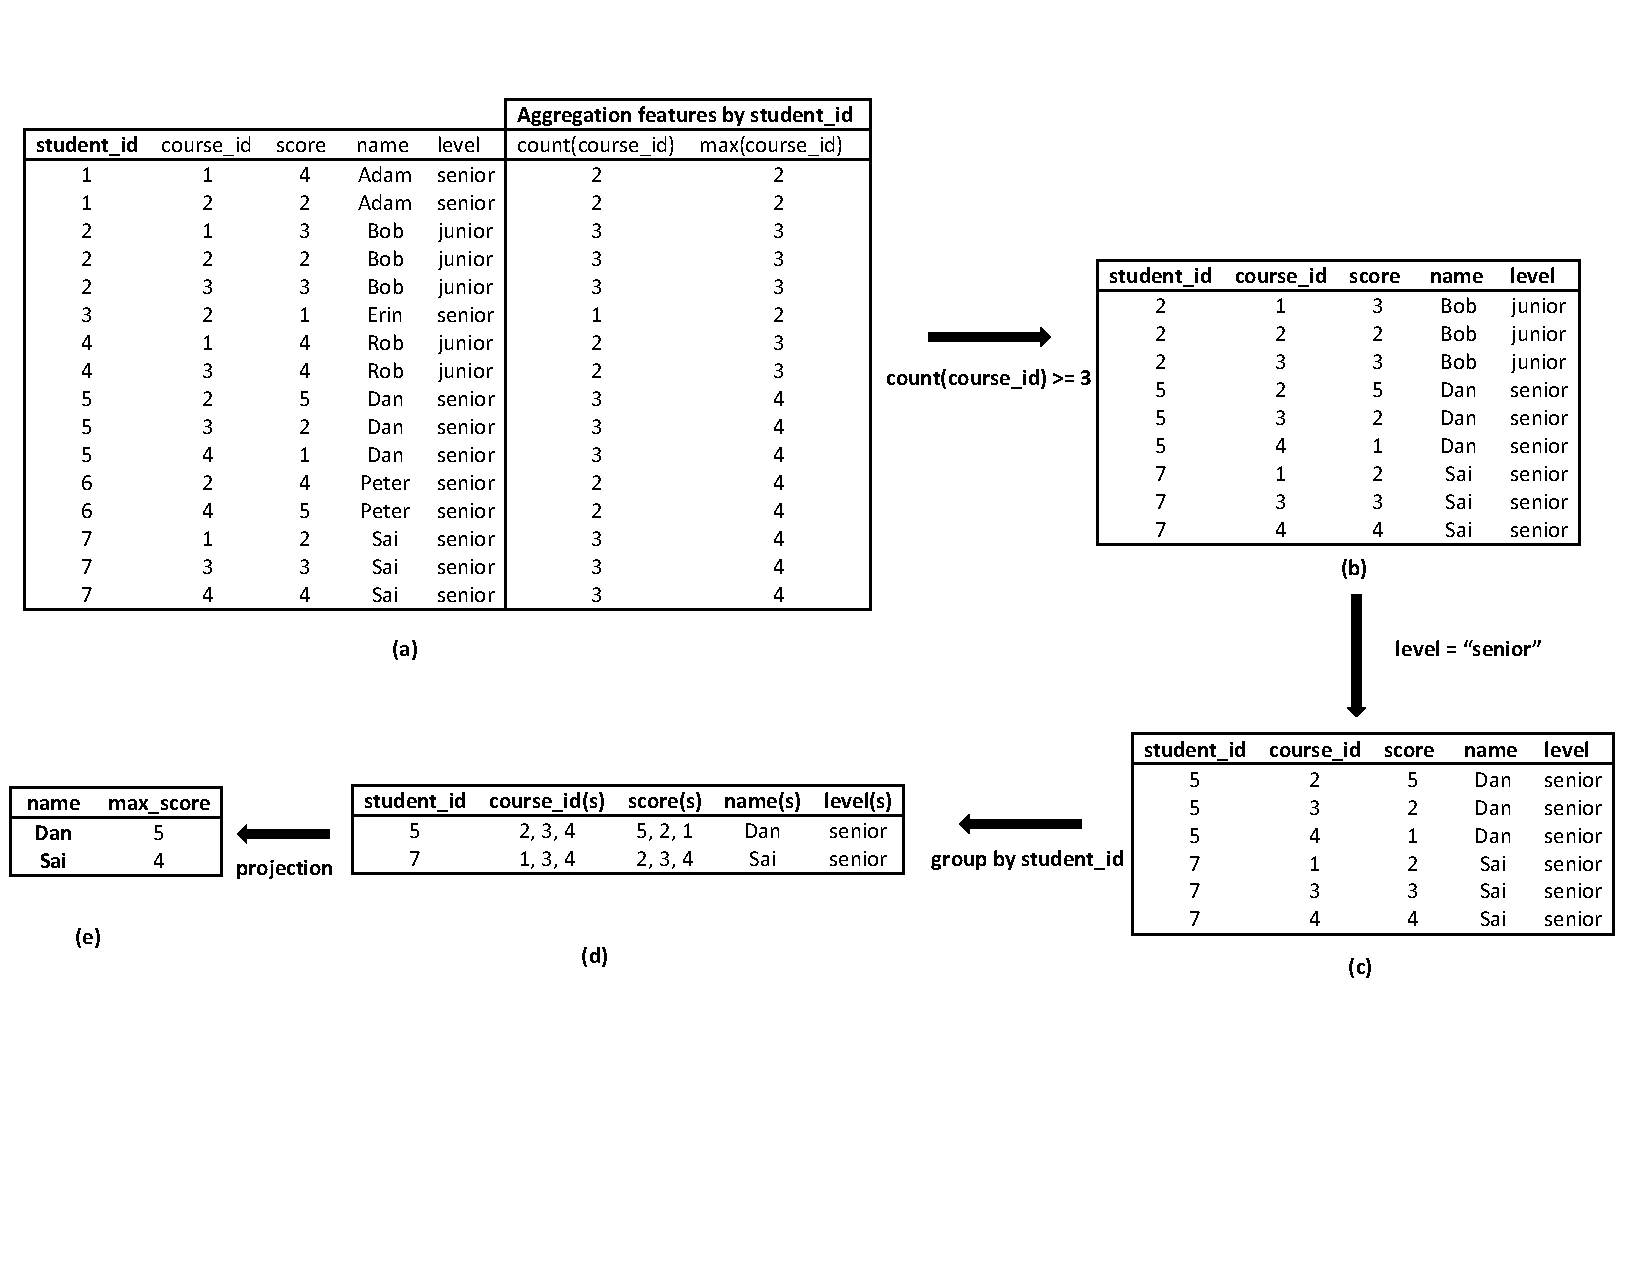
\includegraphics[scale=0.65]{fullexample}
  \vspace*{-1.0ex}\caption {{\label{fig:fullexample}
  Illustration of xxx 
}}

\end{figure*}

In this step, \ourtool takes as input a query skeleton, and
infers the query conditions (Section~\ref{sec:condition}),
aggregates (Section~\ref{sec:agg_search}), and order-by clauses (Section~\ref{sec:orderby}); and finally
produces a set of syntactically-correct SQL queries.

%The SQL skeleton produced by the first step, though incomplete,
%serves as a good reference in inferring complete and valid SQL queries.
%In this step, our technique the remaining incomplete parts: conditions and
%aggregates, by rule-based learning and type-directed search, respectively.

\subsubsection{Inferring Query Conditions}
\label{sec:condition}

\ourtool casts the problem of \textit{query condition inference} as finding
appropriate \textit{rules} that can perfectly divide the whole searching space
into positive part and negative part. In our context, the search space
contains all tuples generated by joining the input tables; the positive part
are all tuples in the output table; and the negative part are the rest
tuples.

A natural way to learn rules is using a decision-tree-based
learning algorithm to infer a set of rules as query conditions. However,
a key challenge to effectively employ the decision tree algorithm is how to devise
expressive features. Existing approaches~\cite{Tran:2009} simply use
data values in each tuple as features. Although using data values as
features is sufficent for simple query conditions like
``\CodeIn{student.level = 'senior'}'' , it suffers from losing much useful \textit{structure information}
needed in a SQL query, and fails to infer complex query conditions
like ``\CodeIn{count(enrolled.course\_id) > 3} (after grouping by
the \CodeIn{student.student\_id} column)''.


\ourtool addresses this challenge by enriching the existing data value features with
two types of additional features:

\begin{itemize}

\item {\textbf{Aggregation Features}}. \ourtool groups the data values
in a table by each column, and applies every aggregate functions (i.e.,
\CodeIn{COUNT}, \CodeIn{MAX}, \CodeIn{MIN} and \CodeIn{AVG})
to compute the values for the other columns. 
\todo{cannot infer group by column1, column2} \todo{add an example}


\item {\textbf{Comparison Features}}. For each tuple, \ourtool compares
the data values of every two type-comparable columns, and records
the comparison results ($1$ or $0$) as features.
\todo{add an example}


\end{itemize}

The above two additional features seamlessly encodes SQL
structure
 knowledge encoding permits our technique
to make use of correlations between columns, rather than only values
from each isolated and sequential columns.
Table~\ref{tbl:com} shows an example.

\todo{The incerasing number of features, can be falsified quickly}

After enriching the original data values with additional features, 
\ourtool uses a variant of the decision tree algorithm, called PART~\cite{Frank:1998},
to infer a set of accurate and expressive rules.
Compared to the original decision tree algorithm~\cite{},
PART has two notable features. \todo{unclear}
First, it uses a ``divide-and-conquer'' strategy to repeatedly
construct rules and remove the tuples that have been covered until no tuples are left,
and thus is more efficient.
Second, when constructing each rule, PART uses a pruned decision tree built from
current set of tuples and only makes the leaf with the largest coverage
into the resulting rules, without keeping the whole learned tree in memory.
This permits PART \todo{what good results?} and is more suitable
for the SQL inference problem.



\begin{figure*}[t]
    \centering
    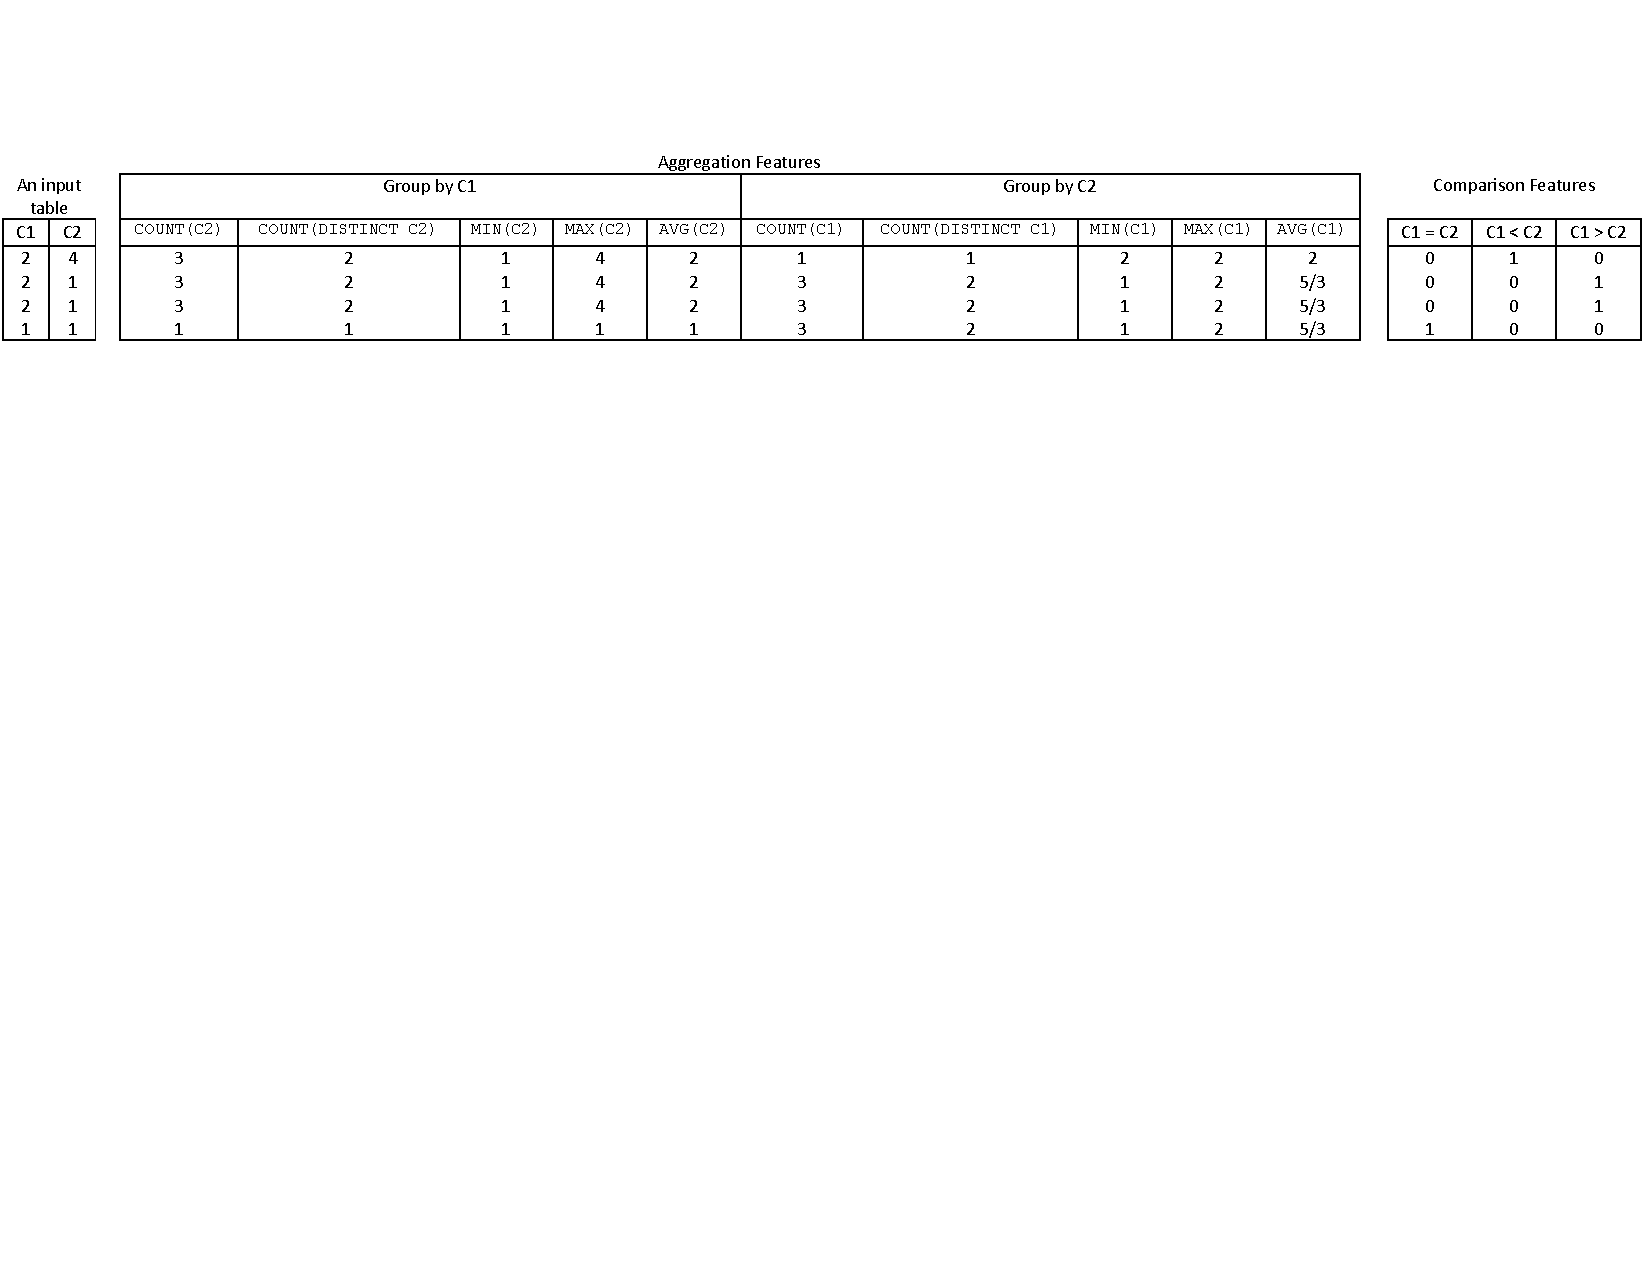
\includegraphics[scale=0.75]{featurex}
	\caption{Illustration of the aggregation features and the comparison
    features enriched by \ourtool. (Left) An example input table with
    two columns: C1 and C2. (Center) The aggregation features enriched by
    \ourtool for the input table. (Right) The comparison features
    enriched by \ourtool for the input table.
}
	\label{tbl:com}
\end{figure*}


Take the joined table in Figure~\ref{fig:motivating} as an example, \ourtool
infers the following rules to perfectly divide the joined table into
the query output:

\smallskip
{
\CodeIn{COUNT(enrolled.course\_id) $>$ 2} (group by \CodeIn{student\_id} )
}

\CodeIn{\&\& student.level =`senior'}.
%\smallskip

\ourtool next splits the inferred rules and put each condition
into the appropriate places in a SQL query (based on the SQL language's
syntax). For the example in Figure~\ref{fig:motivating}, \ourtool
extracts \CodeIn{\&\& student.level =`senior'} as the query
condition, treats \CodeIn{student\_id} as the group by column,
and uses \CodeIn{COUNT(enrolled.course\_id) $>$ 2}
in the \CodeIn{Having} clause.




%\end{itemize}

\subsubsection{Searching for Aggregates}
\label{sec:agg_search}

For each column produced by an aggregation operator,
the whole search space includes all possible combinations
of table columns and the five supported aggregation operators (see Figure~\ref{fig:syntax}).
\ourtool leverages the following two observations to
further reduce the search space:

\begin{itemize}
\item The data type of an output column must be compatible with the
aggregation operator's return type. For instance, if an output column
has the String type, it must not use aggregation operators (e.g.,
\CodeIn{count} and \CodeIn{sum}) that returns
an Integer. 

\item If an arithmetic aggregation operator, such as \CodeIn{max} and \CodeIn{min},
is used, each value in the output column must has appeared in the input table.
\end{itemize}

%In our experience, the type-directed searching strategy significantly reduces the
%searching space and makes our tool find the desirable aggregates faster.

%\todo{Order by structure, relatively each to add}
\subsubsection{Searching for Order By Columns}
\label{sec:orderby}

After the query conditions and aggregates are inferred,
\ourtool observes data values in each output table column. If
the data values in a column appear are sorted, \ourtool
append the column name to the \CodeIn{Order By} clause.
